\section{Technical Implementation and Details}

\subsection{FIDO2}

As already briefly introduced in \autoref{subsec:fido_alliance}, the \gls{fido}2 project is a joint efforts of the \gls{w3c} and the \gls{fido} alliance. It consists of the \gls{js} standard, the \wa{}, and the \glsfirst{ctap}. The \wa{} is standardized and managed by the \gls{w3c}, while the \gls{ctap} is authored by the \gls{fido} alliance. However, the \gls{fido} alliance also initially developed the \wa{} under the name \gls{fido} 2.0 before officially handing it over to the \gls{w3c}.\footcites[See][254]{Schwartz2018}[See][3]{FormalVerificationWebAuthn}

\begin{figure}[hbt]
	\centering
	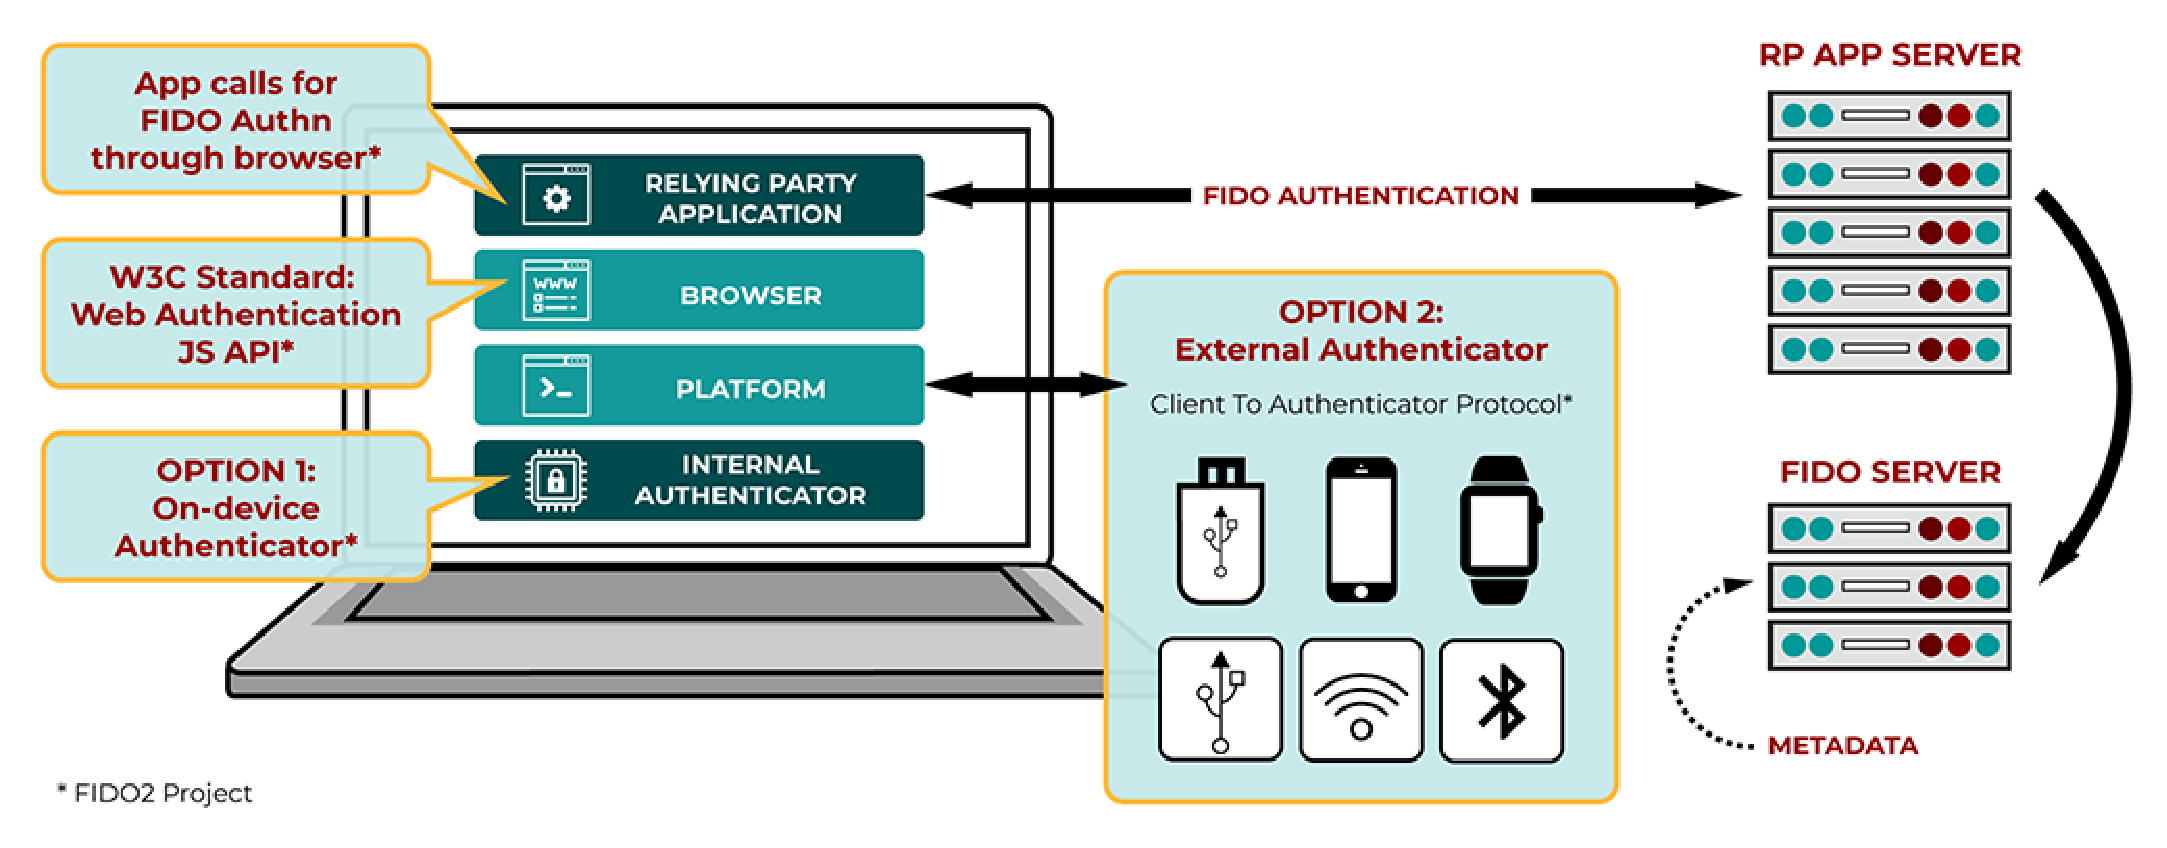
\includegraphics[width=\textwidth]{pics/FIDO2-Graphic-v2.eps}
	\caption[\gls{fido}2 architecture overview]{\gls{fido}2 architecture overview\footnotemark}
	\label{fig:fido2_architecture}
\end{figure}
\footnotetext{Source: https://fidoalliance.org/specifications/, last access on 09/14/2019}

\autoref{fig:fido2_architecture} shows the overview of the \gls{fido}2 project. A noteworthy change is the possibility to use either a \textit{roaming}, i.e., external authenticator or an authenticator that is built into the device.

\subsection{Client to Authenticator Protocol 2}

The \glsfirst{ctap} 2 is based on the \gls{u2f} protocol version 1.2 and defines three parts:

\begin{enumerate}
	\item the authenticator \gls{api}
	\item message encoding
	\item transport-specifc binding
\end{enumerate}

The key methods of the authenticator \gls{api} are explained in more detail below. Message encoding describes the process of encoding the corresponding message in a binary encoding called \gls{cbor} that is suitable for, e.g., the transport over \gls{ble}, because plain text string and \gls{json} objects can be too big for a transport over such protocols. The transport-specific bindings define the required transformation and bindings in order to comply with the transport protocol specifications.\footcites[See][4--5]{ctap2}

An important difference between \gls{ctap}2 and the preceding standard \gls{u2f} is the fact that \gls{ctap}2 describes only the communication between the client, i.e., web browser and the authenticator, as opposed to \gls{u2f} where the standard also defines the \gls{js} \gls{api} in order to communicate with the authenticator. \autoref{fig:ctap_vs_u2f} shows this architectural difference.\footcites[See][51]{kim-new-way-fido}[See][254]{Schwartz2018}

\begin{figure}[hbt]
	\centering
	\includesvg[width=\textwidth,pretex=\relscale{0.8}]{pics/svg/ctap_vs_u2f}
	\caption[Architectural differences between \gls{u2f} and \gls{ctap}2]{Architectural differences between \gls{u2f} and \gls{ctap}2\footnotemark}
	\label{fig:ctap_vs_u2f}
\end{figure}
\footcitetexts[Source: diagram by author, based on][4]{u2f-overview}[][Chapter 6]{w3c}

\subsubsection{Registration}

The registration procedure calls the method \textit{authenticatorMakeCredential}. The input parameters are identical to the ones defined in the higher level \wa{} and are further explained in \autoref{subsec:wa}. Upon reception of the required data, the authenticator first checks if the \textit{excludeList} if a credential ID is listed that is already registered on the authenticator. This prevents that a user registers multiple accounts. If the user verification or presence option is passed, the authenticator has to ensure a legitimate user is present. Upon successful user verification the authenticator generates a new credential key-pair for the specified algorithm.\footcites[See][9]{ctap2}

After that, the authenticator generates the attestation object consisting of the authentication data, which contain the hash of the \gls{rp} ID, a counter, flags if the user has been verified, and the public key with its unique credential ID. Besides that, the authenticator also sends the attestation statement if required. This statement can for example be issued by the \gls{tpm}, Android Key attestation, or the private attestation key of the authenticator token.\footcites[See][9]{ctap2}[See][Chapter 8]{w3c}

\subsubsection{Authentication and transaction confirmation}

Authentication is performed by using the method \textit{authenticatorGetAssertion} of the \gls{ctap} protocol. Again the higher level \wa{} defines the input parameters. The identifier of the \gls{rp} is sent to the authenticator and optionally a list of allowed public keys the authenticator is allowed to retrieve. After optional user verification and presence detection the authenticator displays the data to the user if it has a display to do so. When these checks succeeded, the authenticator accesses the corresponding credentials.\footcites[See][11-13]{ctap2}

The authenticator generates an assertion signature over the received hash of the client data and the authenticator data which consist of the hashed \gls{rp} ID, the flags for user presence and verification, a counter, and the attested credential data. The attested credential data comprises of the \gls{aaguid}, credential ID and the credential public key.\footcites[See][Chapter 6.4.1.]{w3c}

\subsubsection{Factory reset}

As the \gls{uaf} protocol, but in contrast to the \gls{u2f} specification, the \gls{ctap} does define a method to completely factory reset the authenticator in order to de-register every user account on it. To avoid accidental deletion of all user accounts, the protocol specifies that the authenticator may ask for user confirmation. However, it is not possible to delete a specific user account.\footcites[See][26]{ctap2}

\subsection{Web Authentication API}
\label{subsec:wa}

The \gls{api} defined in the \wa{} is actually an extension of the Credential Management \gls{api}, which is another \gls{api} in development, but currently in a draft state.\footnote{The \gls{w3c} standardization process can be viewed in the \autoref{sec:w3c-process}} The Credential Management \gls{api} defines \textit{navigator.credentials} property with the \textit{create} and \textit{get} methods and has the goal to offer an \gls{api} for programmatically accessing the user agent's password storage capabilities. The \wa{} is adding further method overloads to support public-key based credentials, too.\footcites[See][Chapter 1]{w3c}[See][Chapter 1.1]{w3c-credentials}

Authentication and registration in the context of the \wa{} are a special form of network protocols, called a \textit{ceremony}. A ceremony is the concept of extending a network protocol to include human nodes, too. This allows the specification to take the human factor into account, too.\footcite[See][2]{Ellison2007CeremonyDA}

The \wa{} is backwards compatible to the \gls{u2f} compatible, thus making every security token that is usable for \gls{u2f} compatible with the \wa, too. However, a crucial restriction of the legacy \gls{u2f} protocol in usage with \gls{fido}2 is, that it is only usable as a second factor and not for passwordless logins.

\subsubsection{Registration}

A new key-pair for the registration with a \gls{rp} is generated by calling the asynchronous method \textit{navigator.credentials.create} with an object that contains the required \textit{publicKey} property. The publicKey object contains the ID and name of the \gls{rp} and the user information consisting of a username, optional display name and and a unique ID. Given the fact that, e.g., the authenticator stores the ID value, it should not consist of any information that can be linked to the user. Further, the publicKey object contains a random challenge generated by server to prevent replay attacks.\footcites[See][Chapter 5.1.3]{w3c}

Besides that, with the public key credential parameters (\textit{pubKeyCredParams}) array it is possible to define the desired algorithm that should be used for the key-pair generation. The algorithm (\textit{alg}) IDs are obtained from the \gls{iana} registry of \gls{cose} algorithms. The ID -7 expands to \gls{ecdsa} with \gls{sha}-256, while -257 denotes that the \gls{rsa} algorithm should be used in conjunction with \gls{sha}-256. The order in the array denotes the preferred but also accepted fallback algorithms.\footcites[See][Chapter 5.3, 11.3]{w3c}

Additionally, the \gls{rp} can define a list of credentials to exclude (\textit{excludeCredentials}) to, e.g., prevent the user from creating multiple key-pairs that are registered with the \gls{rp}. Furthermore a \textit{timeout} value can be specified in which the operation should succeed or fail.\footcites[See][Chapter 5.4]{w3c}

Moreover, the \gls{rp} can set the \textit{authenticatorSelection} which defines the requirement if a user needs to be verified (\frqq required\flqq, \frqq preferred\flqq, \frqq discouraged\flqq), the option if the credentials need to be stored on the authenticator (\frqq requireResidentKey\flqq), and the authenticator attachment modality, i.e., if the authenticator should be platform specific or a cross-platform (roaming) authenticator.\footcites[See][Chapter 6.2.1]{w3c}

Finally, the \textit{attestation} is of importance. The \gls{rp} can specify either a direct, indirect, or none attestation. None means that the \gls{rp} is not interested in the attestation of the authenticator. A direct attestation requires a signed attestation statement generated by the authenticator to verify its authenticity. In contrast, an indirect attestation leaves the authenticator in charge how to generate the attestation certificate. The authenticator may use a per-origin \gls{ca} to protect the users privacy.\footcites[See][Chapter 5.4.6]{w3c}

\begin{example}{Exemplary Web Authentication API registration}{listing:webauthnreg}
\begin{minted}[breaklines]{javascript}
const publicKeyOptions = {
  challenge: 'Wings2019', // normally random string from the server in binary form (Uint8Array)
  rp: {
    name: 'Web Authn Test',
    id: 'https://timbrust.de'
  },
  user: {
    id: 'C0E3F2BFCFA8179F', // usually in binary form (Uint8Array)
    name: 'me@timbrust.de',
    displayName: 'tim'
  },
  pubKeyCredParams: [{ alg: -7, type: 'public-key' }],
  authenticatorSelection: {
    authenticatorAttachment: 'cross-platform'
  },
  timeout: 600,
  attestation: 'none'
};

const credential = await navigator.credentials.create({
  publicKey: publicKeyOptions
});
\end{minted}
\end{example}

\autoref{listing:webauthnreg} shows an example payload for the registration of a new credential with the \wa{} with the previously introduced parameters. The publicKeyOptions payload can now be passed to the authenticator by calling the authenticatorMakeCredential method. The client passes the user and \gls{rp} to the authenticator. Further, it is evaluated if the authenticator should verify the user or if a check of user presence is sufficient. For this evaluation the property \textit{userVerification} is used. Besides that, the list of credentials to exclude, the public key credential parameters and the hash of the client data is provided to the authenticator. The client data comprises of the server provided challenge, it's origin and the string type \textit{webauthn.create}.

Upon reception of the \textit{attestationObject} and included credential ID in it, the client can generate the credential to be returned to the \gls{rp}, as shown in \autoref{listing:webauthnregresp}.
\\
\begin{example}{Web Authentication API registration response}{listing:webauthnregresp}
\begin{minted}[breaklines]{javascript}
const credential = {
  id: 'BShOCQ2c32dv4aqyy3oWmcu_9s4tz0VIob81U5tg [...]',
  rawId: ArrayBuffer(59),
  response: {
    clientDataJSON: ArrayBuffer(121),
    attestationObject: ArrayBuffer(306)
  },
  type: 'public-key'
};
\end{minted}
\end{example}

The created credential consists of an ID, both as a string and binary reprenstation, the type that is always \textit{public-key} and the \textit{response} object. The response object is constructed from the returned \textit{attestationObject} and the client data.
\\
\begin{example}{Web Authentication API registration client data}{listing:webauthnregrespclientdata}
\begin{minted}[breaklines]{javascript}
const clientDataJSON = {
  challenge: 'Wings2019',
  origin: 'https://timbrust.de',
  type: 'webauthn.create'
};
\end{minted}
\end{example}

\autoref{listing:webauthnregrespclientdata} shows the decoded client data from the \wa{} registration response from \autoref{listing:webauthnreg}. The data contains the challenge sent by the \gls{rp} and the origin of the \gls{rp}. Each registration is flagged with the type of \textit{webauthn.create}.

In contrast, the attestation sent from the authenticator is much bigger. On the first hierarchy it contains the attestation statement format identifier (\textit{fmt}), such as packed, tpm, or fido-u2f, the attestation statement (\textit{attmStmt}, and the authentication data (\textit{authData}). The authentication data includes the evaluated user flags, for instance if the user was present or verified, a signature counter if supported by the authenticator, and the hash of the \gls{rp} ID. In detail, the attested credential data of the authentication data contains the public key ID, the public key itself, e.g., the public point on an \gls{ec} and the \gls{aaguid} if attestation is. not set to none, otherwise 16 zero bytes.

\begin{example}{Web Authentication API registration attestation}{listing:webauthnregrespattestation}
\begin{minted}[breaklines]{javascript}
const attestationObject = {
  fmt: 'fido-u2f',
  attStmt: {
    sig: '[...]',
    x5c: []
  },
  authData: {
    rpIdHash: '068a7ad7f858dadbf691af6f2f7ca86d4dee5a080b [...]',
    flags: {
      userPresent: true,
      reserved1: false,
      userVerified: false,
      reserved2: '0',
      attestedCredentialData: true,
      extensionDataIncluded: false
    },
    signCount: 0,
    attestedCredentialData: {
      aaguid: '0000000000000000',
      credentialIdLength: 96,
      credentialId: ArrayBuffer(59), // identical to publicKeyCredential.id
      credentialPublicKey: {
        kty: 'EC',
        alg: 'ECDSA_w_SHA256',
        crv: 'P-256',
        x: 'xHxgcBFgJolQ5lvukADki+cUzTPcmk50tfj0YGH3nYE=',
        y: 'W1OKIxfc6pIE/ANeTD7MqnNVjBXd0L7We9xZ3Hx6nD8='
      }
    }
  }
};
\end{minted}
\end{example}

\subsubsection{Authentication}

An authentication ceremony is started by calling the method \textit{navigator.credentials.get}.
\\
\begin{example}{Exemplary Web Authentication API authentication}{listing:webauthnauth}
\begin{minted}[breaklines]{javascript}
const publicKeyOptions = {
  challenge: 'Wings2019Auth', // normally a random string from the server in binary form (Uint8Array)
  allowCredentials: [
    {
      id: 'BShOCQ2c32dv4aqyy3oWmcu_9s4tz0VIob81U5tg [...]',
      type: 'public-key',
      transports: ['usb', 'ble', 'nfc']
    }
  ],
  timeout: 6000
};

const assertion = await navigator.credentials.get({
  publicKey: publicKeyOptions
});
\end{minted}
\end{example}

\begin{example}{Web Authentication API authentication response}{listing:webauthnauthresp}
\begin{minted}[breaklines]{javascript}
const assertion = {
  id: 'BShOCQ2c32dv4aqyy3oWmcu_9s4tz0VIob81U5tg [...]',
  rawId: ArrayBuffer(59),
  response: {
    authenticatorData: ArrayBuffer(191),
    signature: ArrayBuffer(59),
    clientDataJSON: {
      challenge: 'Wings2019 Auth',
      origin: 'https://timbrust.de',
      type: 'webauthn.get'
    }
  },
  type: 'public-key'
};
\end{minted}
\end{example}